\chapter{Kết quả thực nghiệm}
\ifpdf
    \graphicspath{{Chapter3/Chapter3Figs/PNG/}{Chapter3/Chapter3Figs/PDF/}{Chapter3/Chapter3Figs/}}
\else
    \graphicspath{{Chapter3/Chapter3Figs/EPS/}{Chapter3/Chapter3Figs/}}
\fi
Thực nghiệm trên 2 bộ dữ liệu Binary-class và multi-class
\section{Dữ liệu thực nghiệm}
	Bộ dữ liệu UMICH SI650 (Binary class)
		\begin{itemize}[label = \textbullet]
			\item Binary class
			\item Xây dựng bởi Đại Học Michigan
			\item Gồm 7086 câu được gán nhãn 0(negative) hoặc 1(positive)
			\begin{itemize}[label =  \textendash]
				\item Training dataset: 5000 câu
				\item Test dataset: 2086 câu.
			\end{itemize}
		\end{itemize}
	Bộ dữ liệu Rotten Tomatoes movie review (multi-class)
		\begin{itemize}[label = \textbullet]
			\item Multi class
			\item Xây dựng bởi Pang và L.Lee
			\item Gồm 150000 câu được gán nhãn từ 0 đến 4
			\begin{itemize}[label =  \textendash]
				\item Training dataset: 140000 câu
				\item Test dataset: 10000 câu.
			\end{itemize}
		\end{itemize}
\section{Môi trường thực nghiệm}
\begin{itemize}[label = \textbullet]
		\item Hệ điều hành ubuntu 14.04-64 bit
		\item Intel core i7 - 3540M, CPU 3.0Ghz x 4
		\item Ngôn ngữ lập trình: python
		\item Thư viện hỗ trợ: Tensorflow
	\end{itemize}
\section{Kết quả}
So sánh giá trị hàm Loss giữa Standard-RNN vs LSTM trên bộ dữ liệu multi-class
	\begin{center}
	  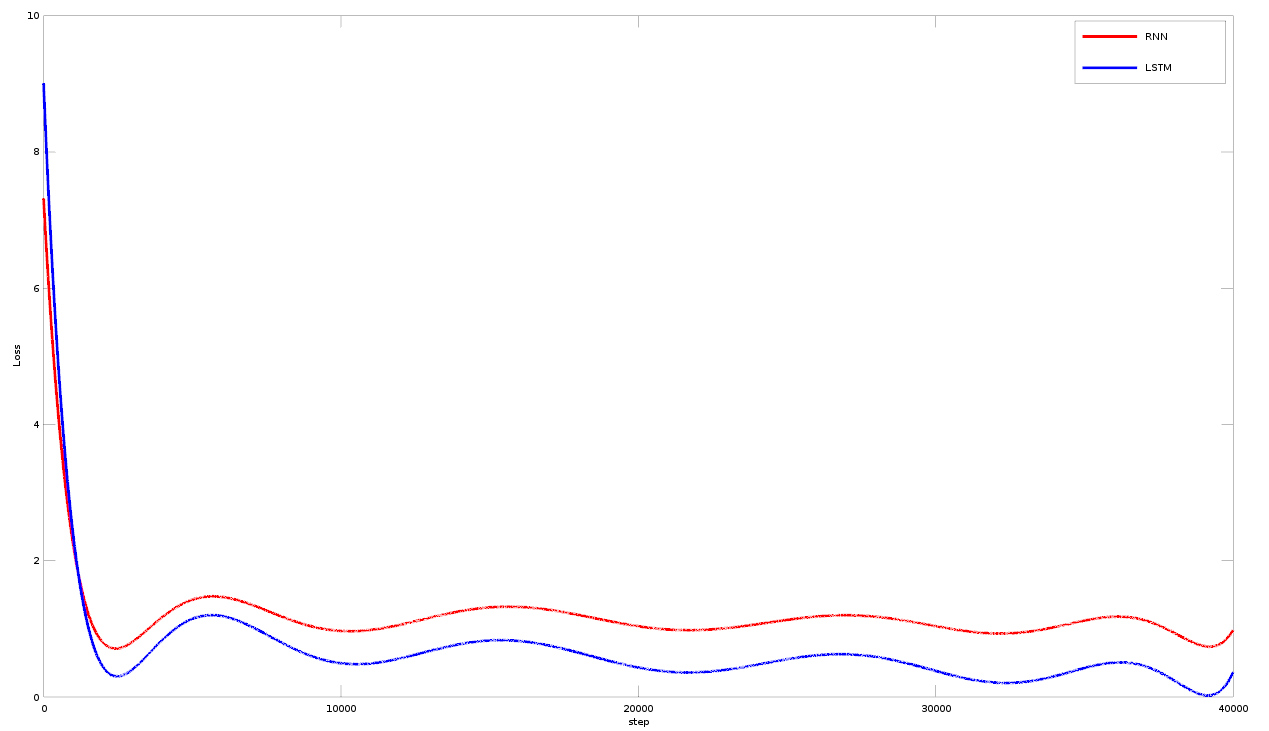
\includegraphics[width=0.8\textwidth]{plot}
	  \captionof{figure}{Đồ thị hàm loss giữa Standard-RNNs vs LSTMs}  
	  \label{plot}
	\end{center}
Kết quả cho thấy mô hình LSTM có khả năng học tốt hơn so với RNNs \\
So sánh kết quả giữa Standard-RNN vs LSTM trên 2 bộ dữ liệu. 
\begin{center}
\begin{tabular}{|c|c|c|c|c|}
\hline
 &\multicolumn{2}{c|}{Binary-class} & \multicolumn{2}{c|}{Multi-class}  \\
\cline{2-5}
 & Traing data & Test data & Training data & Test data  \\
\hline
S-RNN & 98,76\% & 95,12\% &65,62\% & 55,50\% \\
\hline
LSTM & 99,34\% &97,56\% &85,93\% & 62,96\%  \\
\hline
% etc. ...
\end{tabular}
\end{center}
Với bộ binary-class, kết quả thu được khá tốt. Còn với bộ Multi-class, trên tập huấn luyện LSTMs cho kết quả khá tốt, tuy nhiên trên tập test kết quả thu được chưa được tốt. Cần có một mô hình phù hợp hơn với bộ dữ liệu này. 



